\documentclass[12pt,letterpaper]{article}
\usepackage{fullpage}
\usepackage[top=2cm, bottom=4.5cm, left=2.5cm, right=2.5cm]{geometry}
\usepackage{amsmath,amsthm,amsfonts,amssymb,amscd}
\usepackage{lastpage}
\usepackage{enumerate}
\usepackage{fancyhdr}
\usepackage{mathrsfs}
\usepackage{xcolor}
\usepackage{graphicx}
\usepackage{listings}
\usepackage{hyperref}

\hypersetup{%
  colorlinks=true,
  linkcolor=blue,
  linkbordercolor={0 0 1}
}
 
\renewcommand\lstlistingname{Algorithm}
\renewcommand\lstlistlistingname{Algorithms}
\def\lstlistingautorefname{Alg.}

\lstdefinestyle{Python}{
    language        = Python,
    frame           = lines, 
    basicstyle      = \footnotesize,
    keywordstyle    = \color{blue},
    stringstyle     = \color{green},
    commentstyle    = \color{red}\ttfamily
}

\setlength{\parindent}{0.0in}
\setlength{\parskip}{0.05in}

% Edit these as appropriate
\newcommand\course{CSE 3500}
\newcommand\hwnumber{1}                  % <-- homework number
\newcommand\NetIDa{netid19823}           % <-- NetID of person #1
\newcommand\NetIDb{netid12038}           % <-- NetID of person #2 (Comment this line out for problem sets)

\pagestyle{fancyplain}
\headheight 35pt
\lhead{\NetIDa}
\lhead{Daiki Shirafuji\\daikish@kth.se}                 % <-- Comment this line out for problem sets (make sure you are person #1)
\chead{\textbf{\Large Assignment 1}}
\rhead{DD2434 MLadv 2019 \\ \today}
\lfoot{}
\cfoot{}
\rfoot{\small\thepage}
\headsep 1.5em

\begin{document}

\section*{Grade-E Level}


\section*{Question 1}
First, assuming the distribution of samples as a \textit{Gaussian form}
is a sensible choice as the following reason:

\begin{itemize}
  \item 
  According to Central Limit Theorem, the features, which are assumed i.i.d,
  converge into normal distributions.
  \item
  Therefore, the noise also tends to be a normal distribution. 
  \item
  The conditions on \textit{the likelihood} are giving $f$ and $x_i$,
  so that it just depends on the noise, whose distribution may be a normal distribution.
\end{itemize}

Therefore, it is natural to assume that
the distribution of \textit{the likelihood} is a normal distribution.

Second, 
\textit{the assumptions we make by this choice (Gaussian form)}
is that all of features $x_i$ are i.i.d.

Finally, by choosing a spherical covariance matrix for the likelihood,
the assumption is that
a spherical covariance matrix for the likelihood means that the off-diagonal correlations are $0$,
which means features are independent to all other features.

\section*{Question 2}

According to $P(X, Y) = P(Y | X)P(X)$,
the answer is following:

\begin{equation}
\begin{split}
p \left({\textbf{T}| f, X} \right)& = p(t_1|f, X)p(t_2, \ldots, t_N | t_1, f, X) \\
& = p \left ({t_1 | f, X} \right)
*\prod_{i=2}^{N} p\left ({t_i | t_1, \ldots, t_{i-1}, f, X} \right).
\end{split}
\end{equation}



\section*{Question 3}

According to $\epsilon \sim N(\textbf{0}, \sigma^2 \textbf{I})$,
$p(\textbf{T} | \textbf{X}, \textbf{W})$ is following:

\begin{equation}
\begin{split}
p(\textbf{T} | \textbf{X}, \textbf{W}) = \prod_{i=1}^{N - 1} p(t_i | x_i, \textbf{W})
\end{split}
\end{equation}

where $p(t_i | x_i, \textbf{W}) = N(\textbf{W}x_i, \sigma^2 \textbf{I})$.



\section*{Question 4}

\begin{itemize}
  \item 
  What would be the effect of encoding the preferred model with $L_1$ norm (for model parameters)?
\end{itemize}

When encoding with $L_1$ norm instead of $L_2$ norm,
the prior become \textit{\textbf{less}} smooth
because of the variable selection in $L_1$ norm.


\begin{itemize}
  \item 
  Discuss how these two types of priors affect the posterior from the regularisation  perspective. Write down the penalization term, i.e. the negative log-prior, and illustrate for a two-dimensional problem (in the two-dimensional parameter space).
\end{itemize}

First, according to Bayesian Rule, we can say that:
\begin{equation}
\begin{split}
posterior \propto likelihood * prior
\end{split}
\end{equation}

and this is equivalent to:
\begin{equation}
\begin{split}
ln(posterior) \sim ln(likelihood) + ln(penalty).
\end{split}
\end{equation}

This is how these priors affect the posterior as penalties.

Now, start to write down the penalisation term
(i.e. $ln(penalty)$ or $ln(prior)$):
\begin{equation}
\begin{split}
-ln[p(\textbf{W} | \textbf{D})] = &
\frac{1}{2} \sum_{n=1}^{N} (t_n - \textbf{w}^Tf(\textbf{x}_n))^2
+ \frac{\lambda}{2}  \sum_{i=1}^{K} |w_i|^q + const
\end{split}
\end{equation}
where $\textbf{D}$ is the data,
$K$ is the number of elements in one of \textbf{W} row,
$q$ is an integer  value (0, 1, ...), 
and $const$ is a constant value.

In the $L_1$ case, $q$ is $1$,
and in the $L_2$ case, $q$ is $2$.


\begin{figure}[htb]
\centering
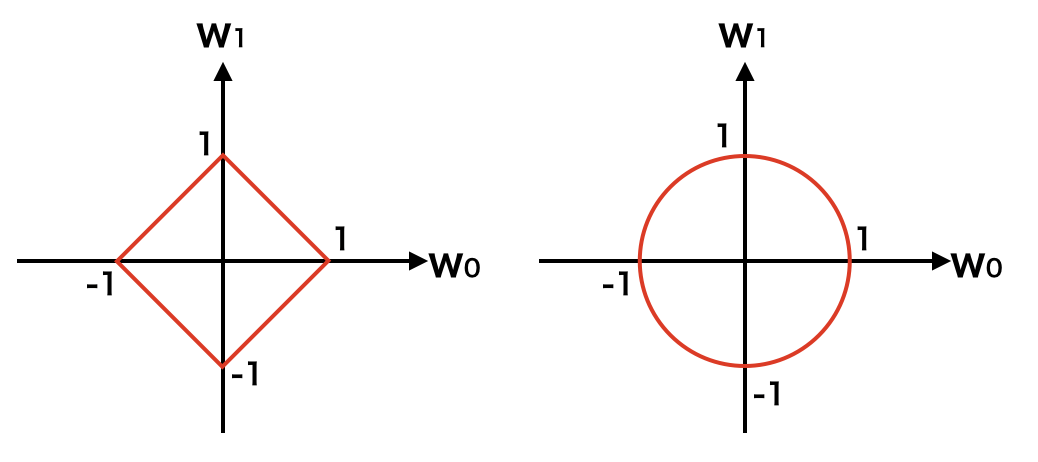
\includegraphics[scale =0.5]{L1and2.png} 
\caption{Regularisation on L1 (left) and L2 (right)}
\end{figure}

Finally, the regularisation in the two-dimensional parameter space are shown in Figure 1.

As Figure 1 is shown,
L1 regularisation tend to yield more sparse solution than L2.



\section*{Question 5}
According to Question 3,
$p(\textbf{T} | \textbf{X}, \textbf{W}) = \prod_{i=1}^{N - 1} p(t_i | x_i, \textbf{W})$
and $p(t_i | x_i, \textbf{W}) = N(\textbf{W}x_i, \sigma^2 \textbf{I})$,
where $i = {1, ..., N}$.
The distribution which is produced by Gaussian forms Gaussian distribution, so that it can be said that:

\begin{equation}
\begin{split}
p(\textbf{T}|\textbf{X}, \textbf{W}) = N(\textbf{W}\textbf{X}, \sigma^2 \textbf{I}).
\end{split}
\end{equation}

The definition of a Gaussian distribution is represented with following:
\begin{equation}
\begin{split}
N(\mu, \Sigma)=\frac{1}{\sqrt{2\pi\Sigma}}exp(\frac{-1}{2}(x-\mu)^T\Sigma^{-1}(x-\mu))
\end{split}
\end{equation}

Now, we set $\Sigma$ as $\tau^2$. Then, according with
$p(\textbf{W})=MN(\textbf{W}_0, \textbf{I}, \tau^2\textbf{I})$,

\begin{equation}
\begin{split}
p(\textbf{W})&=\frac{1}{\sqrt{2\pi\Sigma}}exp(\frac{-1}{2}(W-W_0)^T\Sigma^{-1}(W-W_0)) \\
p(\textbf{T}|\textbf{X}, \textbf{W})& = \frac{1}{\sqrt{2\pi\sigma^2}}exp(\frac{-1}{2\sigma^2}(T-XW)^T(T-XW)).
\end{split}
\end{equation}

In addition, according to Bayesian rule, $p(\textbf{W} | \textbf{T}, \textbf{X}) \propto p(\textbf{W}) * p(\textbf{T}|\textbf{X}, \textbf{W})$.
Therefore, the posterior can be derived with the following:

\begin{equation}
\begin{split}
p(\textbf{W} | \textbf{T}, \textbf{X})& \propto 
\frac{1}{\sqrt{2\pi\Sigma}}exp(\frac{-1}{2}W^T\Sigma^{-1}W)\frac{1}{\sqrt{2\pi\sigma^2}}exp(\frac{-1}{2\sigma^2}(T-XW)^T(T-XW)) \\
& \propto exp(\frac{-1}{2}W^T\Sigma^{-1}W + \frac{-1}{2\sigma^2}(T-XW)^T(T-XW))\\
& = exp(-\frac{1}{2}W^T\Sigma^{-1}W - \frac{1}{2\sigma^2}T^TT + \frac{1}{\sigma^2}T^T(XW) - \frac{1}{2\sigma^2}(XW)^T(XW)).
\end{split}
\end{equation}

Finally, the posterior is formulated with Equation (9).
Next, we explain this posterior in terms of the mean $\mu_W$ and the covariance $\Sigma_W$. 
$p(\textbf{W} | \textbf{T}, \textbf{X})$ can be formulated with $\mu_W$ and $\Sigma_W$ as following:

\begin{equation}
\begin{split}
p(\textbf{W} | \textbf{T}, \textbf{X})
= exp(-\frac{1}{2}W^T\Sigma_{W}^{-1}W
+ W^T\Sigma_{W}^{-1}\mu_W -\frac{1}{2}\mu_W^T\Sigma_{W}^{-1}\mu_W).
\end{split}
\end{equation}

Therefore, the mean and the covariance in the posterior is represented with following:

\begin{equation}
\begin{split}
u_W& = (\Sigma^{-1} + \sigma^{-2}\textbf{X}^T\textbf{X})^{-1}
(\sigma^{-2}\textbf{X}^T\textbf{T} + \Sigma^{-1}W_0)\\
\Sigma_{W}& = (\Sigma^{-1} + \sigma^{-2}\textbf{X}^T\textbf{X})^{-1}.
\end{split}
\end{equation}

As we can see from Equation (10) and (11),
the posterior also form Gaussian distribution in Bayesian linear regression.
Therefore, it can be updated after the relevant information has been taken into account.
This is how the posterior form relates to the estimator.

In terms of $Z$,
there is no affect on the solution.
$Z$ is the constant value here,
so that $Z$ will not affect the posterior mean and the covariance.
$Z$ only represents the evidence, which we are interested in during the model selection.

\section*{Question 6}
In Gaussian Process,
the prior represents a probability distribution over the functions,
not over the parameters.

The choice of this prior is nice
because the function, which is used in Gaussian Process, is not clear usually.

Now, the prior can be represented with $p(f |\textbf{X}, \theta) = N (\textbf{0}, k(\textbf{X}, \textbf{X}))$ according to Equation (11), which is given from the questions.
And $k(\textbf{X}, \textbf{X})$ is given from the following:

\begin{equation}
\begin{split}
k(\textbf{x}_n, \textbf{x}_m) = 
\theta_0 exp(-\frac{\theta_1}{2}||\textbf{x}_n - \textbf{x}_m||^2)
+\theta_2 + \theta_3 \textbf{x}_n^T \textbf{x}_m.
\end{split}
\end{equation}

Samples from the prior is shown in Figure 2, which is quoted from Bishop pp 308.

According with this Figure, the parameters $\theta$ represents how $\theta$ control the shape of the function.
Therefore, we can say the choice of this prior is nice.

\begin{figure}[htb]
\centering
\includegraphics[scale =0.3]{Q6.png} 
\caption{Samples from a Gaussian process prior defined by the covariance function. The title above each plot denotes ($\theta_0$, $\theta_1$, $\theta_2$, $\theta_3$).}
\end{figure}


\section*{Question 7}
According to Bayesian Rule,
$p(T, X, f, \theta)$ can be represented with the following equation.

This is because $\textbf{T}$ is conditionally dependent on $\textbf{X}$ and $\theta$ as the Figure 3 shows.

\begin{equation}
\begin{split}
p(\textbf{T}, \textbf{X}, f, \theta) = p(\textbf{T}|f) p(f|\textbf{X},\theta) p(\textbf{X}) p(\theta).
\end{split}
\end{equation}

\begin{figure}[htb]
\centering
\includegraphics[scale =0.3]{Q7.png} 
\caption{Graphical Model}
\end{figure}


\section*{Question 8}
Because $\textbf{T}$ is conditionally dependent on $\theta$ and $\textbf{X}$,
$p(\textbf{T}|\textbf{X}, \theta)$ is generally formulated with the following:

\begin{equation}
\begin{split}
p(\textbf{T}|\textbf{X}, \theta) = 
\int_{}{} p(\textbf{T}|f) p(f|\textbf{X}, \theta) df
\end{split}
\end{equation}

where $p(f|\textbf{X}, \theta)$ is the prior over the data $\textbf{X}$.
Now, the prior of all $\textbf{X}$ over all $f$ is averaged.


The \textbf{uncertainty} of the value from $f$ and the true value
is represented with $p(\textbf{T}|f)$.
In addition, $p(f|\textbf{X},\theta)$ represents the uncertainty of $\textbf{X}$ and $f$.
Now, we know that these two uncertainties, which are represented from $p(\textbf{T}|f)$ and $p(f|\textbf{X},\theta)$, do "filter" the uncertainty of the inputs $\textbf{X}$ and the values $\textbf{T}$.


In Gaussian Process, we get the average over all functions $f$.
Now, $\theta$ is a constant value in the process of averaging over $f$.
Therefore, $\theta$ remains after averaging,
so that the final result become a function of $\theta$.



\section*{Question 9}
1. Set the prior distribution over $\textbf{W}$ and visualise it.


\begin{figure}[htb]
\centering
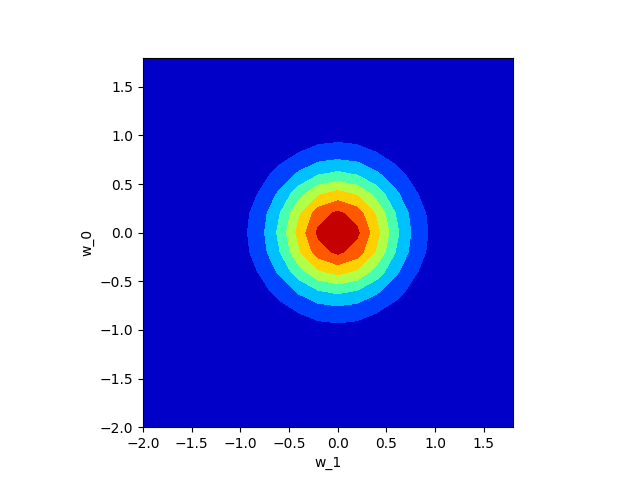
\includegraphics[scale =0.5]{Q9_01.png} 
\caption{The Prior Distribution over \textbf{W}}
\end{figure}

2. Pick a single data point $(x,t)$ and visualise the posterior distribution over $\textbf{W}$.

3. Draw $5$ samples from the posterior and plot the resulting functions.

\begin{figure}[ht]
\begin{tabular}{cc}
\begin{minipage}[t]{0.4\hsize}
\centering
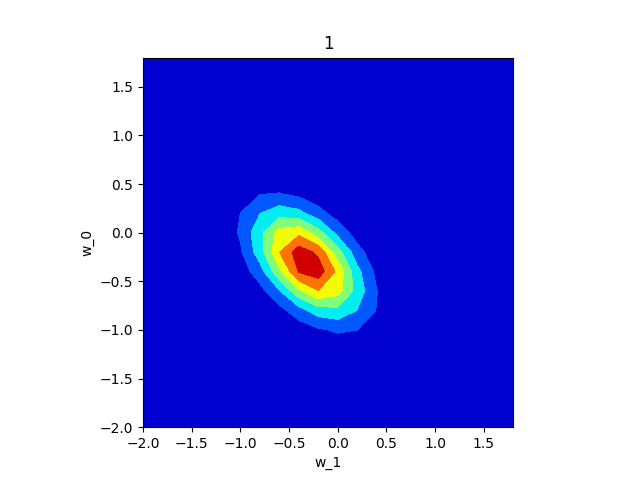
\includegraphics[keepaspectratio, scale=0.4]{Q9_02.png}
\caption{Posterior (1 Observation)}
\end{minipage} &
\begin{minipage}[t]{0.41\hsize}
\centering
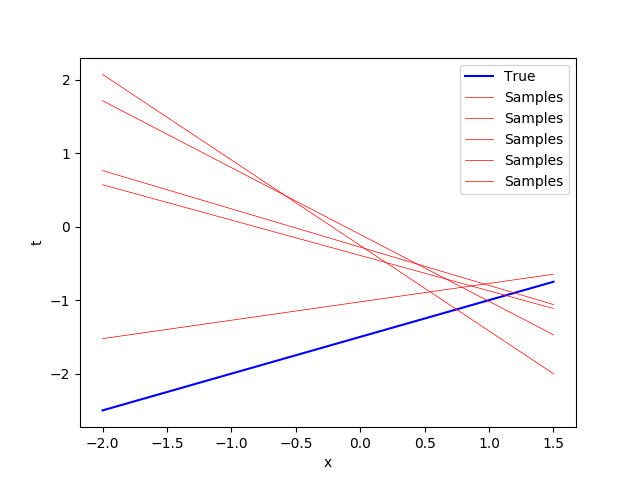
\includegraphics[keepaspectratio, scale=0.41]{Q9_03.png}
\caption{Five Samples from Posterior}
\end{minipage}
\end{tabular}
\end{figure}

4. Repeat $2$ to $3$ by adding additional data points up to $7$.

Answers are shown in the following figures (Figure 7 to Figure 12).
The numbers of adding additional data points are
3, 5, and 7.

\begin{figure}[ht]
\begin{tabular}{cc}
\begin{minipage}[t]{0.4\hsize}
\centering
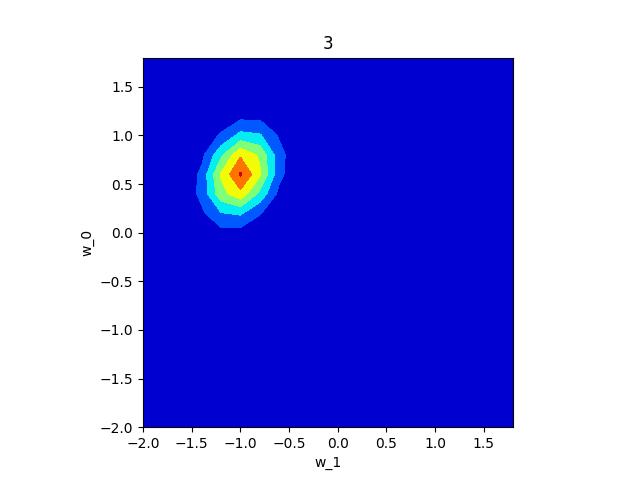
\includegraphics[keepaspectratio, scale=0.4]{Q9_04.png}
\caption{Posterior (3 Observations)}
\end{minipage} &
\begin{minipage}[t]{0.41\hsize}
\centering
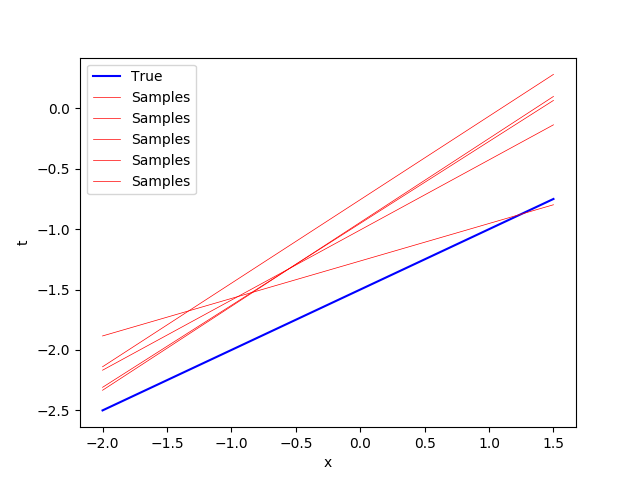
\includegraphics[keepaspectratio, scale=0.41]{Q9_05.png}
\caption{Five Samples from Posterior}
\end{minipage}
\end{tabular}
\end{figure}

\begin{figure}[ht]
\begin{tabular}{cc}
\begin{minipage}[t]{0.4\hsize}
\centering
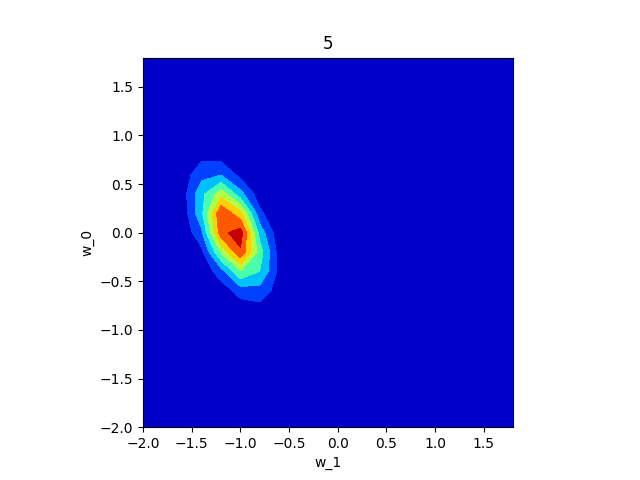
\includegraphics[keepaspectratio, scale=0.4]{Q9_06.png}
\caption{Posterior (5 Observations)}
\end{minipage} &
\begin{minipage}[t]{0.42\hsize}
\centering
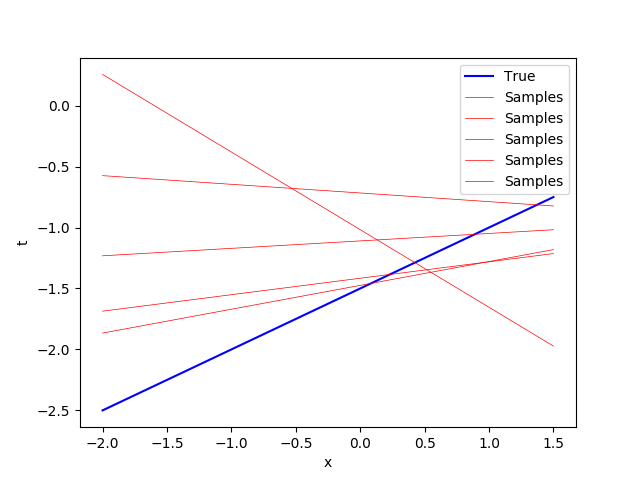
\includegraphics[keepaspectratio, scale=0.42]{Q9_07.png}
\caption{Five Samples from Posterior}
\end{minipage}
\end{tabular}
\end{figure}


\begin{figure}[ht]
\begin{tabular}{cc}
\begin{minipage}[t]{0.4\hsize}
\centering
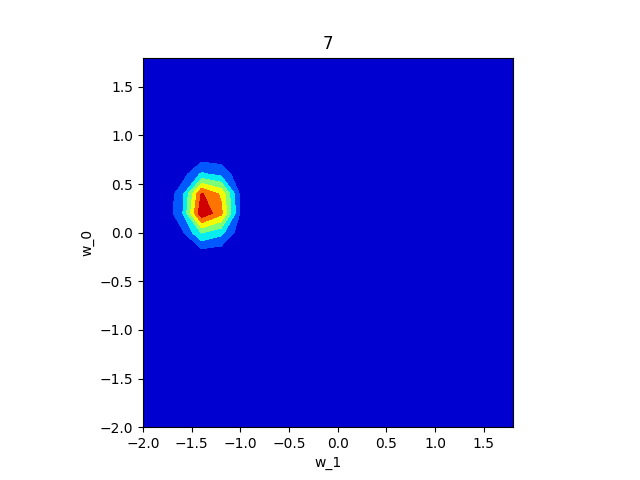
\includegraphics[keepaspectratio, scale=0.4]{Q9_08.png}
\caption{Posterior (7 Observations)}
\end{minipage} &
\begin{minipage}[t]{0.42\hsize}
\centering
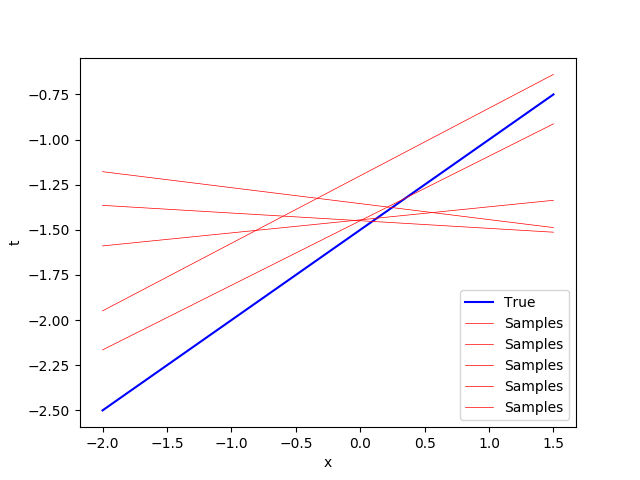
\includegraphics[keepaspectratio, scale=0.42]{Q9_09.png}
\caption{Five Samples from Posterior}
\end{minipage}
\end{tabular}
\end{figure}

\clearpage

5. Given the plots explain the effect of adding more data on the posterior as well as the functions. How would you interpret this effect?

The more the data is,
the samples can represent closer function to the True Function.

This can be explained with the reason that
the more data points we have in advance,
the data points converge into True points.


6. Finally, test the exercise for different values of $\sigma$ e.g. $0.1$, $0.4$ and $0.8$. How does your model account for data with varying noise levels? What is the effect on the posterior?

The results when $\sigma = 0.1$, $0.4$, and $0.8$
(under the condition of 7 Observations)
are shown in the following figures (Figure 13 to Figure 18).

If the noise levels on data are high (i.e. sigma is a large value),
the posterior tends to take a large range in the 2-dimensional space.
This means that it becomes unpredictable in the models.

\begin{figure}[htb]
\centering
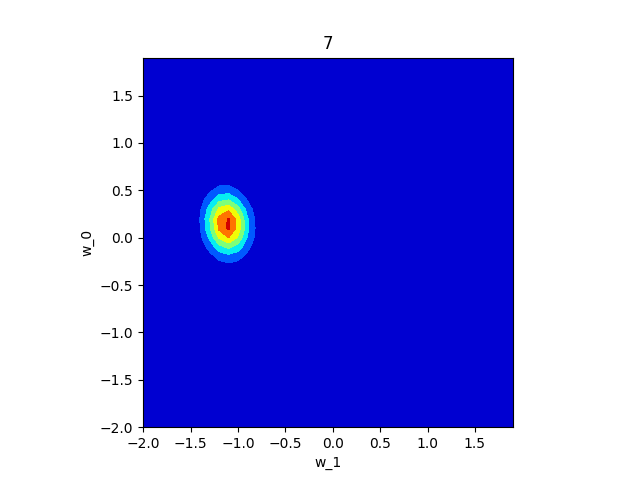
\includegraphics[scale =0.3]{Q9_sigma_01_1.png} 
\caption{Posterior (7 Observations) on $sigma = 0.1$.}
\end{figure}
\begin{figure}[htb]
\centering
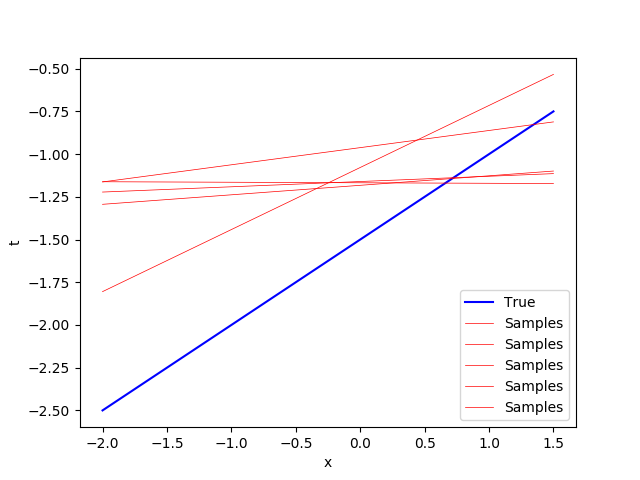
\includegraphics[scale =0.3]{Q9_sigma_01_2.png} 
\caption{The Prior Distribution over \textbf{W} on $sigma = 0.1$.}
\end{figure}
\begin{figure}[htb]
\centering
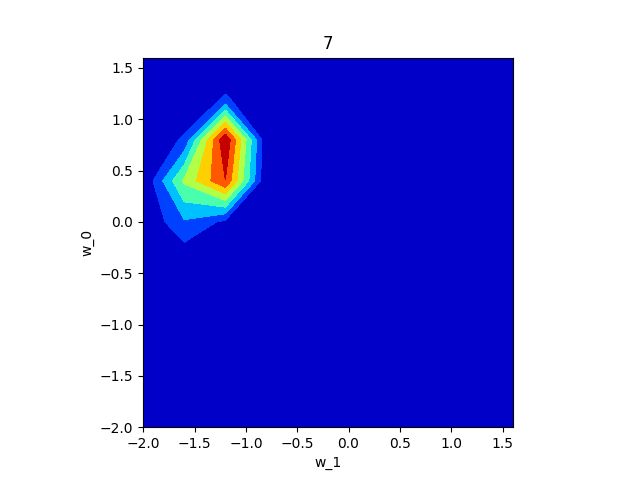
\includegraphics[scale =0.3]{Q9_sigma_04_1.png} 
\caption{Posterior (7 Observations) on $sigma = 0.4$.}
\end{figure}
\begin{figure}[htb]
\centering
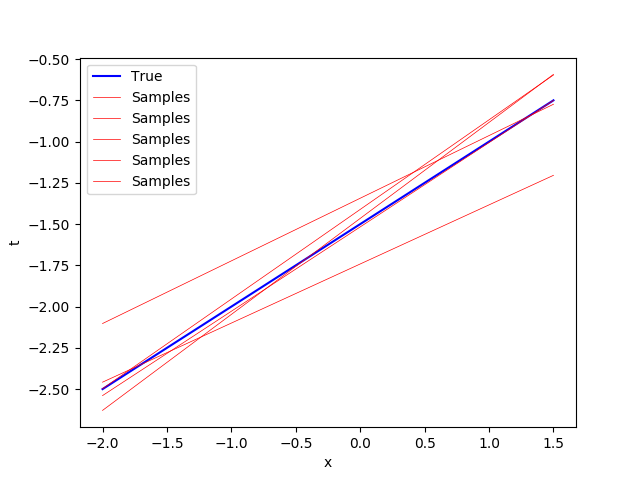
\includegraphics[scale =0.3]{Q9_sigma_04_2.png} 
\caption{The Prior Distribution over \textbf{W} on $sigma = 0.4$.}
\end{figure}
\begin{figure}[htb]
\centering
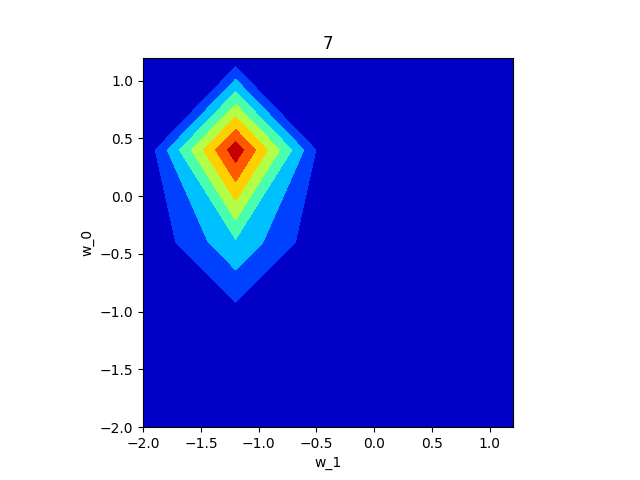
\includegraphics[scale =0.3]{Q9_sigma_08_1.png} 
\caption{Posterior (7 Observations) on $sigma = 0.8$.}
\end{figure}
\begin{figure}[htb]
\centering
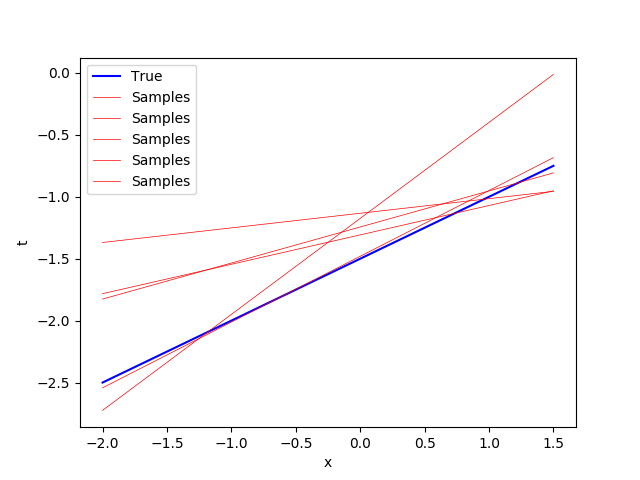
\includegraphics[scale =0.3]{Q9_sigma_08_2.png} 
\caption{The Prior Distribution over \textbf{W} on $sigma = 0.8$.}
\end{figure}

\clearpage

\section*{Question 10}
For each 4 different length scales (0.1, 1, 10, and 100),
10 samples from the prior are shown in the following figures
(Figure 19 to Figure 22).

From these figures,
we can know that 
the samples, which are gotten from the results, show more smooth carve
when the length scales become bigger.


\begin{figure}[htb]
\centering
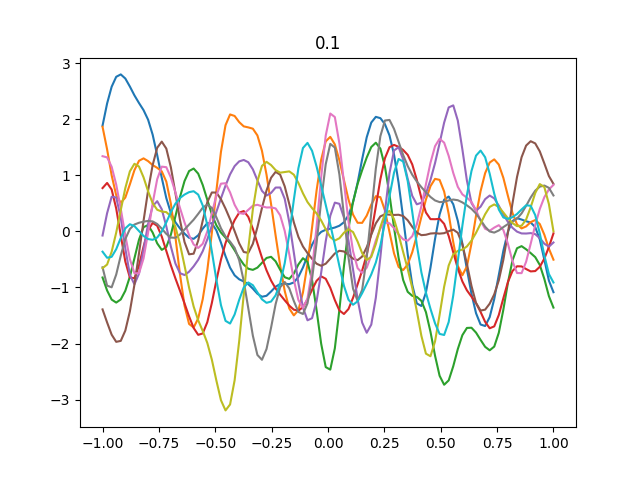
\includegraphics[scale =0.5]{Q10_01.png} 
\caption{10 Samples from GP when length-scale = $0.1$.}
\end{figure}
\begin{figure}[htb]
\centering
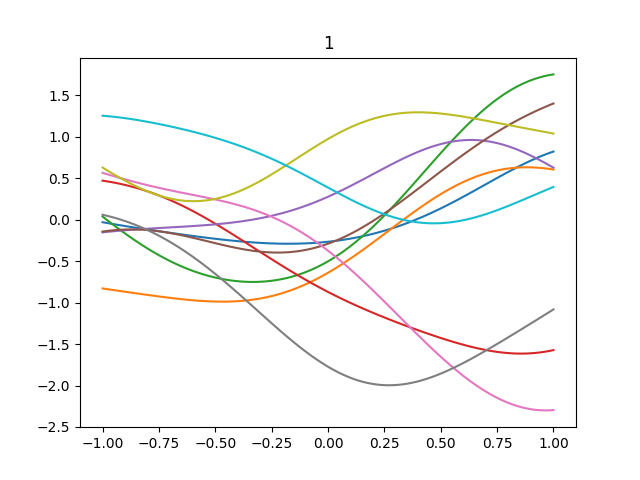
\includegraphics[scale =0.5]{Q10_1.png} 
\caption{10 Samples from GP when length-scale = $1$.}
\end{figure}

\clearpage

\begin{figure}[htb]
\centering
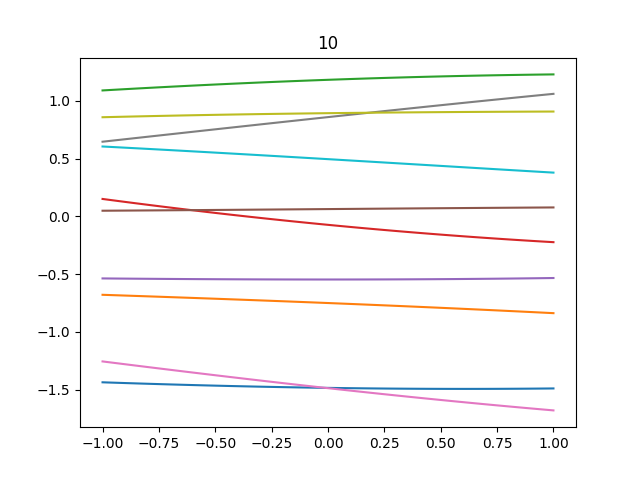
\includegraphics[scale =0.5]{Q10_10.png} 
\caption{10 Samples from GP when length-scale = $10$.}
\end{figure}
\begin{figure}[htb]
\centering
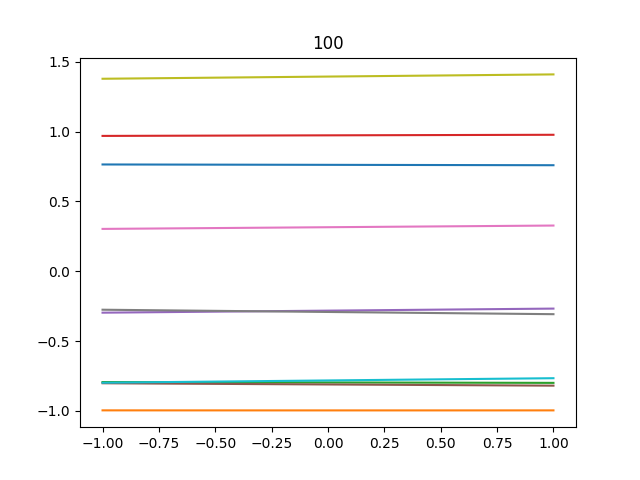
\includegraphics[scale =0.5]{Q10_100.png} 
\caption{10 Samples from GP when length-scale = $100$.}
\end{figure}

\section*{Question 11}
\subsection*{1. What is the posterior before we observe any data?}

Before we observe any data,
we have no information for the posterior in advance,
so that we set the posterior as the value of the prior.
Therefore, the posterior is represented with the following formula:

\begin{equation}
\begin{split}
p(\textbf{f}|\textbf{X}, \theta) = 
N (0, k(\textbf{X}, \textbf{X})).
\end{split}
\end{equation}


\subsection*{2. Compute the predictive posterior distribution of the model.}

We now compute the predictive posterior distribution in the general case.

First of all, let me set that
$t_{N+1}$ is a target value to predict under the condition of $x_{N+1}$.
In addition, from Bishop p. 308,
$m(x_{N+1})=\textbf{k}^T \textbf{C}_N^{-1} \textbf{t}$ and
$\sigma^2(x_{N+1}) = c-\textbf{k}^T \textbf{C}_N^{-1} \textbf{k}$
are defined,
where $c = k(x_{N+1},x_{N+1}) + \beta^{-1}$ and
\begin{equation}
\begin{split}
\textbf{C}_{N+1}=\left(
    \begin{array}{cc}
      \textbf{C}_N & \textbf{k} \\
      \textbf{k}^T & c
    \end{array}
  \right).
\end{split}
\end{equation}


The predictive posterior distribution can be represented with $p(t_{N+1}|\textbf{t}_N)$,
and the joint distribution $p(\textbf{t}_{N+1})$ can be represented with
$N(t_{N+1}|0, \textbf{C}_{N+1})$.

Therefore, the predictive posterior distribution is represented with following:

\begin{equation}
\begin{split}
p(t_{N+1}|\textbf{t}) = N(t_{N+1}|m(x_{N+1}), \sigma^2(x_{N+1}))
\end{split}
\end{equation}



\subsection*{3. Sample from this posterior with points both close to and far away from the observed data. Explain the observed effects.}

As shown in the following figure (Figure 23), we can say that
as the samples is closer to the observed data,
the samples are converged into it.
On the other hand, we can also say that
when the samples go away from the observed data,
the samples tend to be not able to be controllable.

\begin{figure}[htb]
\centering
\includegraphics[scale =0.5]{Q11_01.png} 
\caption{Observations with length-scale = $1$ (Noise included).}
\end{figure}


\subsection*{4. Plot the data, the predictive mean and the predictive variance of the posterior from the data.}

The required figure is shown in the following figure (Figure 24).

\begin{figure}[htb]
\centering
\includegraphics[scale =0.5]{Q11_02.png} 
\caption{With noises in a diagonal covariance matrix to the squared exponential.}
\end{figure}


\subsection*{5. Compare the samples of the posterior with the ones from the prior. Is the observed behavior desirable?}

Comparing the samples of the posterior with the ones from the prior,
we can know that
the difference between  the prior and the posterior is that 
the samples are collected more or not.
This behaviour is desirable because it relate to the model information.


\begin{figure}[htb]
\centering
\includegraphics[scale =0.5]{Q11_03.png} 
\caption{Length-scale=3.}
\end{figure}



\subsection*{6. What would happen if you added a diagonal covariance matrix to the squared exponential?}

We know from comparing Figure 25 with the following figure (Figure 26) that
when we added the noise to a diagonal covariance matrix to the squared exponential,
it become more difficult to predict the True Function than without noises.


\begin{figure}[htb]
\centering
\includegraphics[scale =0.5]{Q11_04.png} 
\caption{Adding noises in a diagonal covariance matrix to the squared exponential (Length-scale=3).}
\end{figure}


\end{document}
